\documentclass[17pt]{article}

\usepackage[margin=1in, paperwidth=8.5in, paperheight=11in]{geometry}
\usepackage{amsmath}
\usepackage[document]{ragged2e}
\usepackage{graphicx}
\usepackage{listings}
\usepackage{color}
\usepackage[none]{hyphenat}

\definecolor{dkgreen}{rgb}{0,0.6,0}
\definecolor{gray}{rgb}{0.5,0.5,0.5}
\definecolor{mauve}{rgb}{0.58,0,0.82}

\lstset{frame=tb,
  language=Python,
  aboveskip=3mm,
  belowskip=3mm,
  showstringspaces=false,
  columns=flexible,
  basicstyle={\small\ttfamily},
  numbers=none,
  numberstyle=\tiny\color{gray},
  keywordstyle=\color{blue},
  commentstyle=\color{dkgreen},
  stringstyle=\color{mauve},
  breaklines=true,
  breakatwhitespace=true,
  tabsize=3
}

\begin{document}

\title{{Bayesean Data Analysis - Exercise 8}}
\maketitle


\section{Model assessment: LOO\_CV for factory data with Stan}

\subsection{Separate model}
Here is that Stan code for the separate model:

\begin{lstlisting}
data {
    int<lower=0> N; // number of data points
    int<lower=0> K; // number of groups
    int<lower=1,upper=K> x[N]; // group indicator
    vector[N] y; //
}

parameters {
    vector[K] mu;         // group means
    vector<lower=0>[K] sigma;
}

model {
  y ~ normal(mu[x], sigma[x]);
}

generated quantities {
    real ypred;
    vector[N] log_lik;
    
    ypred = normal_rng(mu[6], sigma[6]);
    
    for (i in 1:N)
        log_lik[i] = normal_lpdf(y[i] | mu[x[i]], sigma[x[i]]);
}
\end{lstlisting}


If the PSIS-LOO value is considered to be stable, then lower PSIS-LOO value is considered to be better. \\
The separate model has PSIS-LOO value of -132.133 which is the worst of all the models. \\~\\

The effective number of parameters is: 9.69, which means that 9 parameters are considered to be effective. \\~\\

Below is the histogram of the $ \hat{k} $ values for the separate model

\begin{center}
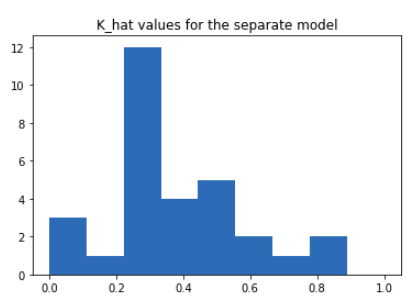
\includegraphics[width=10cm, height=7cm]{separate_model.png}
\end{center}

There are 3 $ \hat{k} $ values that are greater than 0.7 which means that the PSIS-LOO value is not completely accurate and better methods should be used for evaluation of those values.



\subsection{Hierarchical model}
Here is that Stan code for the hierarchical model:

\begin{lstlisting}
data {
    int<lower=0> N; // number of data points
    int<lower=0> K; // number of groups
    int<lower=1,upper=K> x[N]; // group indicator
    vector[N] y; //
}

parameters {
    real mu0;             // prior mean
    real<lower=0> sigma0; // prior std
    
    vector[K] mu;         // group means
    real<lower=0> sigma;
}

model {
    mu ~ normal(mu0, sigma0);
    y ~ normal(mu[x], sigma);
}

generated quantities {
    real mu7;
    real ypred6;
    vector[N] log_lik;
    
    mu7 = normal_rng(mu0, sigma0);
    ypred6 = normal_rng(mu[6], sigma);
    
    
    for (i in 1:N)
        log_lik[i] = normal_lpdf(y[i] | mu[x[i]], sigma);    
}
\end{lstlisting}


If the PSIS-LOO value is considered to be stable, then lower PSIS-LOO value is considered to be better. \\
The hierarchical model has PSIS-LOO value of -126.758 which is the lowest of all the models and this model can be considered to be \textbf{the best}. \\~\\

The effective number of parameters is: 5.662, which means that 5 parameters are confidered to be effective. \\~\\

Below is the histogram of the $ \hat{k} $ values for the hierarchical model

\begin{center}
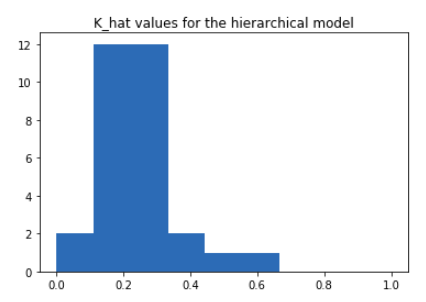
\includegraphics[width=10cm, height=7cm]{hierarchical_model.png}
\end{center}

From the histgram, we can see that all the $ \hat{k} $ values are lower than 0.7, which means that the PSIS-LOO value can be considered to be accurate and reliable.


\subsection{Pooled model}
Here is that Stan code for the pooled model:

\begin{lstlisting}
data {
    int<lower=0> N; // number of data points
    vector[N] y;
}

parameters {
    real mu;             // prior mean
    real<lower=0> sigma;
}

model {
  y ~ normal(mu, sigma);
}

generated quantities {
    real ypred;
    vector[N] log_lik;
    
    ypred = normal_rng(mu, sigma);
    
    for (i in 1:N)
        log_lik[i] = normal_lpdf(y[i] | mu, sigma);   
}
\end{lstlisting}


If the PSIS-LOO value is considered to be stable, then lower PSIS-LOO value is considered to be better. \\
The pooled model has PSIS-LOO value of -130.995 which is the second best model after the hierarchical. \\~\\

The effective number of parameters is: 2.04, which means that 2 parameters are considered to be effective. \\~\\

Below is the histogram of the $ \hat{k} $ values for the pooled model

\begin{center}
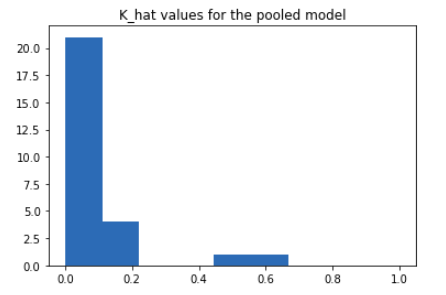
\includegraphics[width=10cm, height=7cm]{pooled_model.png}
\end{center}

From the histgram, we can see that all the $ \hat{k} $ values are lower than 0.7, which means that the PSIS-LOO value can be considered to be accurate and reliable.


\end{document}








